\chapter{Results}

%\section{Experiment setup}

We use~\cite{terada} for sensor specification. The sensors are ZigBee temperature sensors, collecting data at one reading per second. In~\cite{terada}, the authors have used 12~bits for one temperature reading. Therefore, our $SSR$ (sensor data sampling rate) is expected to be 1.25 byte/second. The $SDT$ (sensor data throughput) is taken to be 13.4 kbps~\cite{zigbee}. The MULEs' speed is taken to be 10m/s~\cite{muleSpeed}. The sensor positions are chosen randomly in a field of 1000m~$\times$~1000m, and the sensor range is 50m. Note that Zigbee sensor ranges can lie between 10m to 100m.

\section{Simulation results}
We now present simulation results of our heuristic applied on the following cases:
\begin{itemize}
\item Field size 1000m $\times$ 1000m
\item Sensor Range: 50 m
\item Number of sensors: 50, 60, 70, 80, 90, 100
\end{itemize}

{\bf Comments: You should give an interpretation of what each result
indicates.}

\pagebreak

\subsection{50 sensors}
\begin{figure}[H]
\includegraphics[width=15cm]{50/res_avg.png}
\end{figure}
\begin{figure}[H]
\includegraphics[width=15cm]{50/res_lat.png}
\end{figure}
\subsection{60 sensors}
\begin{figure}[H]
\includegraphics[width=15cm]{60/res_avg.png}
\end{figure}
\begin{figure}[H]
\includegraphics[width=15cm]{60/res_lat.png}
\end{figure}

\subsection{70 sensors}
\begin{figure}[H]
\includegraphics[width=15cm]{70/res_avg.png}
\end{figure}
\begin{figure}[H]
\includegraphics[width=15cm]{70/res_lat.png}
\end{figure}

\subsection{80 sensors}
\begin{figure}[H]
\includegraphics[width=15cm]{80/res_avg.png}
\end{figure}
\begin{figure}[H]
\includegraphics[width=15cm]{80/res_lat.png}
\end{figure}

\subsection{90 sensors}
\begin{figure}[H]
\includegraphics[width=15cm]{90/res_avg.png}
\end{figure}
\begin{figure}[H]
\includegraphics[width=15cm]{90/res_lat.png}
\end{figure}

\subsection{100 sensors}
\begin{figure}[H]
\includegraphics[width=15cm]{100/res_avg.png}
\end{figure}
\begin{figure}[H]
\includegraphics[width=15cm]{100/res_lat.png}
\end{figure}
